\section{Corpus Creation}
\label{cp4:corpus-creation}

Corpus creation consists of three main steps, namely \textit{(1)} selection of tasks, \textit{(2)} selection of artifacts, and \textit{(3)} identification of relevant text within the selected artifacts. We detail each of these steps in the following sections.




\subsection{Software Tasks}
\label{cp4:corpus-tasks}


We consider a software task as a piece of work undertaken by a developer that often has to be finished within a certain time~\cite{2004merriam}.
Two common places a software task can be found are:

\begin{itemize}
    \item the description of a bug or feature request reported in a bug tracking systems; or in
    \item a post in a community forum, development mailing lists, and others.
\end{itemize}

GitHub issues or Stack Overflow (SO) posts are resources promptly available on the Web that align with our task definition.
In fact, several studies have used both as sources for software tasks~\cite{Arya2019, baltes2019, nadi2020, Xu2017}. Nonetheless, the sheer amount of data available on GitHub and Stack Overflow poses challenges to the selection of tasks for our corpus.
Baltes et al.~\cite{baltes2019} argues that even a cursory inspection of a sample set
of Stack Overflow posts shows clear differences in a post's content or structure due to aspects such as programming languages, frameworks, associated technologies, and others.


We scope task selection to
the \textit{Android} development domain as a means to define a common topic from which we can extract tasks from each source. This decision
restricts our selection to a single programming language (\textit{Java})
while it still allows us to investigate a domain that has been
widely discussed by practitioners and researchers alike.
For instance, over 35,000 developers have used Q\&A forums to discuss tasks covering 87\% of the Android API~\cite{parnin2012}
while researchers have investigated how changes to the Android SDK impact its ecosystem and development community~\cite{linares2014, bavota2014b, mcdonnell2013}.


\subsubsection{Stack Overflow tasks}

Provided that we restrict our corpus to tasks related to the Android development domain,
we randomly select 150 SO post from a curated list about Android development~\cite{baltes2019-rep}.


\textit{Saving WebView page to cache}~\cite{so18607655}
is the title of tasks in our corpus extracted from Stack Overflow. In this task, a developer describes the need
to
``\textit{save the website the first time it is connected to the internet so that a further connection is no longer needed}''.
To complete this task, a developer might refer to the Android Webview API~\cite{apiWebView}
or Q\&A forums about the Android cache system~\cite{so8410830}.


\subsubsection{GitHub tasks}

Since we are not aware of a comprehensive dataset of GitHub issues related to Android development, we devised our own strategy to fetch such data.


We selected 15 of top starred Android projects on GitHub by filtering the list of projects to the ones that contained the \textit{Java} and \textit{Android} tags.
For each of these projects, we randomly select 10 issues as the GitHub tasks of our corpus for a total of 150 distinct issues.
While selecting issues, we took care to check that they had at least one follow-up comment and that the issue title did not contain certain words, e.g., {\small \texttt{test}} or {\small  \texttt{ignore}},
so that our selection ignored issues automatically created by scripts or bots---a common pitfall that researchers must be aware of when mining GitHub~\cite{kalliamvakou2014}.




\textit{No lock screen controls ever}~\cite{git3578}
is an example of one of the issues in our corpus extracted from the \texttt{AntennaPod} open-source project.
Although the expected behaviour is that the app controls should be visible even with the screen locked,  a user reports that the app screen is missing.
A developer addressing this issue might review the Android lock task documentation~\cite{apiLockTask}
or refer to examples of applications that use the Android lock screen~\cite{mediumLockApp}.





\subsection{Artifact Selection}
\label{cp4:corpus-artifacts}


Our artifact selection approach seeks to simulate everyday practices on how developers search the Web~\cite{rao2020, Xia2017}. That is, we formulate a query for each task and use a Web search engine to retrieve artifacts that are pertinent to that task.


\subsubsection{Artifact sources}

As there are many different sources of artifacts, we restrict artifact selection to well known and studied sources~\cite{Starke2009,Kevic2014, Li2013}, i.e.,
Android and Java SE API documentation, Github issues, Stack Overflow answers; and Web tutorials or blog posts from Java and Android development.



\subsubsection{Query formulation}



We consider a task's title (i.e., SO question or GitHub issue title) as the seed used to search artifacts
using the \texttt{googlesearch} API~\cite{googlesearch}.
Coming up with proper search terms is a critical step of any search~\cite{Haiduc2013}
and, ideally, we should be able to formulate a query with terms able to retrieve exactly the most pertinent artifacts for a software task.
However, studies have shown that developers perform poorly in identifying good search terms~\cite{Starke2009,Kevic2014, Li2013} and thus, using a task's title
as an educated approximation to terms that a developer might use is a common procedure adopted by many studies in the field (e.g.,~\cite{Xu2017} or ~\cite{Silva2019}).







\subsubsection{Search results}


We fetch a maximum of 5 resources per artifact source --- a limitation necessary due to throttling or even blocking mechanisms in the APIs used to get the content of each source considered. We exclude search results that do not appear in the Amazon Alexa~\cite{alexa} Android Web pages traffic statistics in the period from April 2020 to March 2021. 
While applying this filter potentially decreased the number of artifacts per task, it ensured that results were indeed related to Android development. 
For instance, for a task discussing ``\textit{left and right swap}'' 
filtering avoided fetching unrelated resources, such as a Web page on  ``\textit{stock swap}''.
Table~\ref{tbl:googlesearch-example-git} shows one search result per artifact source for the GitHub task introduced in Section~\ref{cp4:corpus-tasks}.


Processing an artifact's content into a sequence of individual sentences 
followed procedures analogous to other studies in the field~\cite{Arya2019, nadi2020}.
Given a search result \texttt{URL}, we use \texttt{BeautifulSoup}~\cite{beautifulsoup4},
\texttt{StackAPI}~\cite{StackAPI} and \texttt{PyGithub}~\cite{PyGithub}
to fetch the artifacts' content and sentences in each paragraph
were identified using the Stanford CoreNLP toolkit~\cite{CoreNLP}.







\begin{table}[H]
\centering    
\begin{scriptsize}
\begin{threeparttable}
\rowcolors{2}{}{lightgray}    
\begin{tabular}{l|l}

\hline

\multicolumn{2}{c}{\textit{Saving WebView page to cache}}  \\

\hline
\hline

\multirow{1}{*}{API documentation}
& Managing WebView objects - Android Developers \\
% & WebView - Android Developers \\

\multirow{1}{*}{Github issues}
& WebView Caching contents WebView using the cachePolicy \\
% & Investigate whether removing WebView files on erase is a good idea \\


\multirow{1}{*}{StackOverflow answers}
& Android WebView not loading second page from cache \\
% & Save webview content for offline browsing? \\
\hline

\end{tabular}
\end{threeparttable}
\end{scriptsize}
\caption{Sample of artifacts obtained for a StackOverflow task~\cite{so18607655}}
\label{tbl:googlesearch-example-so}
\end{table}



\begin{table}[H]
\centering    
\begin{scriptsize}
\begin{threeparttable}
\rowcolors{2}{}{lightgray}    
\begin{tabular}{l|l}

\hline

\multicolumn{2}{c}{\textit{No lock screen controls ever}}  \\

\hline
\hline

\multirow{1}{*}{API documentation}
& Lock task mode - Android Developers \\
% & Recents Screen - Android Developers \\

\multirow{1}{*}{Github issues}
& Lock screen controls disappear on Android 11 \\
% & Bug: No lock screen image and controls \\


\multirow{1}{*}{StackOverflow answers}
& How to add MediaPlayer controls on lock screen? \\
% & How to disable home button in Android like lock screen apps do? \\



\multirow{1}{*}{Miscellaneous}
& Create A React Native App - Which works on Lock Screen (Android) \\

\hline


\end{tabular}
\end{threeparttable}
\end{scriptsize}
\caption{Sample of artifacts obtained for a Github task~\cite{git3578} }
\label{tbl:googlesearch-example-git}
\end{table}






\subsection{Relevant text detection}
\label{cp4:corpus-relevant-text}




 
We rely on state-of-the-art approaches able to automatically identify relevant text for the tasks and artifacts in our corpus~\cite{nadi2020, Robillard2015, Lotufo2012, Xu2017}.


We systematically reviewed related work and we identified techniques applicable to our domain problem. Selection criteria considered each technique's availability in existing replication packages and their readiness for use.
We also refrained from using approaches with training procedures (e.g., ~\cite{liu2020} or ~\cite{Treude2016}) because of the challenges related to parameter tuning~\cite{Chaparro2017, fucci2019}.



Based on these criteria, three techniques were selected for the following sources:


\begin{itemize}[leftmargin=\parindent, font=\normalfont\itshape]
    \item \texttt{\acs{AnsBot}} (\textit{SO Answers}) uses several features (e.g., information entropy, textual patterns, entity overlap, etc.) to determine that a sentence has useful information to a developer's technical question~\cite{Xu2017}.
    
    \item \texttt{\acs{Krec}} (\textit{API Documentation}) identifies text fragments that reflect ``potentially important text that programmers cannot afford to ignore when using the API''~\cite{Robillard2015}.
    
    \item \texttt{\acs{Hurried}} (\textit{GitHub issues}) identify the most relevant sentences in a bug report based on three factors used to assess a sentence's relevancy (i.e., sentence's prominence in the issue, topic, and its similarity to the task)~\cite{Lotufo2012}.
\end{itemize}


% \art{Do I need to give details for miscellaneous?}

Tables~\ref{tbl:git-example-ansbot} to~\ref{tbl:git-example-hurried}
illustrate sentences selected by each approach\footnote{The number of sentences shown per technique
differs slightly due to a technique's input parameters and the length of the input artifact.}
 for pertinent artifacts retrieved for our Github lock screen task. 
% The techniques precision range from 71\% (\texttt{HurriedBug}) to 90\% (\texttt{APIRef}) and thus, we observe some unrelated sentences,
% such as a sentence expressing gratitude in Table~\ref{tbl:git-example-ansbot}.



\begin{table}[H]
\centering    
\begin{scriptsize}
\begin{threeparttable}
\rowcolors{2}{}{lightgray}
\begin{tabular}{ll}

\hline
\multicolumn{2}{c}{\textit{How to add MediaPlayer controls on lock screen?}} \\
\hline
\hline

1 & \parbox[l][.8cm][c]{10.5cm}{I had the same problem, and well, the solution was simple, do not use any widget, simply use the RemoteControlClientCompat class.} \\
2 & \parbox[l][.8cm][c]{10.5cm}{Here is my lockScreenControls() method code, which I call whenever I want to show this type of control (when plays a song).} \\
3 & \parbox[l][.5cm][c]{10.5cm}{Thank @ianhlake for the good 2 video} \\

\hline


\end{tabular}
\end{threeparttable}
\end{scriptsize}
\caption{Pertinent sentences automatically detected by \acs{AnsBot}}
\label{tbl:git-example-ansbot}
\end{table}

\begin{table}[H]
\centering    
\begin{scriptsize}
\begin{threeparttable}
\rowcolors{2}{}{lightgray}
\begin{tabular}{ll}
    
\hline
\multicolumn{2}{c}{\textit{Lock task mode - Android Developers}} \\
\hline
\hline

1 & \parbox[l][.8cm][c]{10.5cm}{You might use lock task mode if you're developing a kiosk application or a launcher to present a collection of apps.} \\
2 & \parbox[l][.8cm][c]{10.5cm}{To check if the current app is running in lock task mode, use the methods on ActivityManager as shown in the following example:} \\
3 & \parbox[l][.8cm][c]{10.5cm}{You can call KeyguardManager methods to find out if the device is locked and use an Activity lifecycle callback (such as onResume() that's called after unlocking) to start lock task mode.} \\
\hline

\end{tabular}
\end{threeparttable}
\end{scriptsize}
\caption{Pertinent sentences automatically detected by \acs{Krec}}
\label{tbl:git-example-krec}
\end{table}

\begin{table}[H]
\centering    
\begin{scriptsize}
\begin{threeparttable}
\rowcolors{2}{}{lightgray}
\begin{tabular}{ll}

\hline
\multicolumn{2}{c}{\textit{How to add MediaPlayer controls on lock screen?}} \\
\hline
\hline

1 & \parbox[l][.8cm][c]{10.5cm}{I had the same problem, and well, the solution was simple, do not use any widget, simply use the RemoteControlClientCompat class.} \\
2 & \parbox[l][.8cm][c]{10.5cm}{Here is my lockScreenControls() method code, which I call whenever I want to show this type of control (when plays a song).} \\
3 & \parbox[l][.5cm][c]{10.5cm}{Thank @ianhlake for the good 2 video} \\

\hline


\end{tabular}
\end{threeparttable}
\end{scriptsize}
\caption{Pertinent sentences automatically detected by \acs{Hurried}}
\label{tbl:git-example-hurried}
\end{table}





\subsection{Corpus Summary}
\textcolor{white}{force ident} % this is just for the chapter outline



Figure~\ref{fig:corpus-creation-pipeline} summarizes procedures for corpus creation.
We randomly sample a set of Android development tasks from Stack Overflow and GitHub
and use the Google search engine to find potential resources that might have
information for a task. We only consider resources highly ranked at Amazon Alexa and, for these resources, we apply state of the art techniques to detect relevant text in the artifact's content.



Overall, our corpus comprises 300 tasks evenly selected from SO and Git. 
There is a total of 262,278 sentences in 2,586 artifacts pertaining API documentation, Stack Overflow answers, Github issue discussions, and miscellaneous Web tutorials or blog posts. 



\begin{figure}
    \centering
    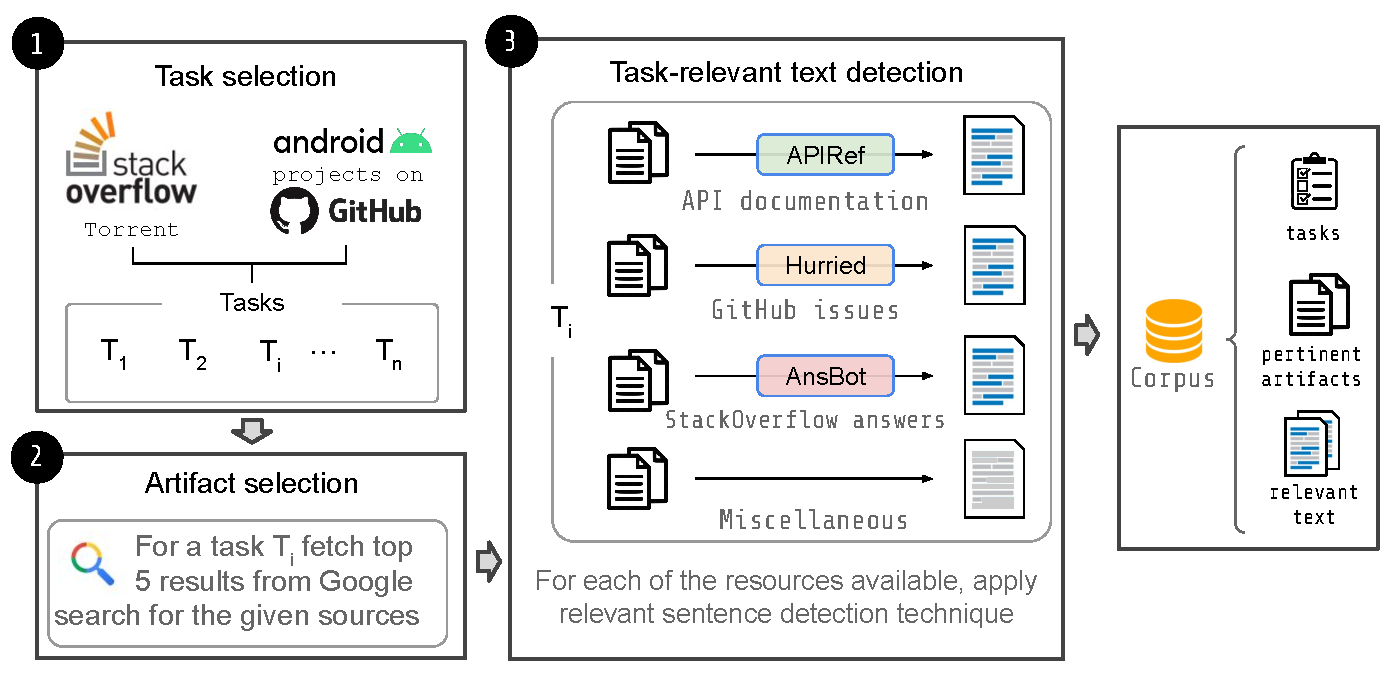
\includegraphics[width=\textwidth]{cp4/corpus-creation-pipeline}
    \caption{Summary of procedures for corpus creation}
    \label{fig:corpus-creation-pipeline}
\end{figure}

